\documentclass[10pt,a4paper,final]{article} %draft

\usepackage[english, russian]{babel}

\usepackage{geometry}
%\usepackage[a4paper,left=2cm,right=2cm,top=2cm,bottom=2cm,bindingo ffset=0cm]{geometry}

\usepackage[T2A]{fontenc}
\usepackage[utf8]{inputenc}

\usepackage[utf8]{inputenc}

\usepackage[final]{pdfpages}

\usepackage{textcomp,enumitem}

\usepackage{amsmath,amsthm,amssymb}

\usepackage{longtable}
\usepackage{array}
\usepackage{adjustbox}




\usepackage{listings}
\usepackage{xcolor}
\usepackage{caption}

\definecolor{codegray}{rgb}{0.95,0.95,0.95}
\definecolor{codepurple}{rgb}{0.58,0,0.82}
\definecolor{codegreen}{rgb}{0,0.5,0} % зеленый цвет
\definecolor{codeblue}{rgb}{0,0,0.5} % синий цвет
\definecolor{codestring}{rgb}{0.64,0.08,0.08} % цвет строк


\lstset{
	language=haskell,
	extendedchars=true,
	literate=
	{а}{{\selectfont\char224}}1
	{б}{{\selectfont\char225}}1
	{в}{{\selectfont\char226}}1
	{г}{{\selectfont\char227}}1
	{д}{{\selectfont\char228}}1
	{е}{{\selectfont\char229}}1
	{ж}{{\selectfont\char230}}1
	{з}{{\selectfont\char231}}1
	{и}{{\selectfont\char232}}1
	{й}{{\selectfont\char233}}1
	{к}{{\selectfont\char234}}1
	{л}{{\selectfont\char235}}1
	{м}{{\selectfont\char236}}1
	{н}{{\selectfont\char237}}1
	{о}{{\selectfont\char238}}1
	{п}{{\selectfont\char239}}1
	{р}{{\selectfont\char240}}1
	{с}{{\selectfont\char241}}1
	{т}{{\selectfont\char242}}1
	{у}{{\selectfont\char243}}1
	{ф}{{\selectfont\char244}}1
	{х}{{\selectfont\char245}}1
	{ц}{{\selectfont\char246}}1
	{ч}{{\selectfont\char247}}1
	{ш}{{\selectfont\char248}}1
	{щ}{{\selectfont\char249}}1
	{ъ}{{\selectfont\char250}}1
	{ы}{{\selectfont\char251}}1
	{ь}{{\selectfont\char252}}1
	{э}{{\selectfont\char253}}1
	{ю}{{\selectfont\char254}}1
	{я}{{\selectfont\char255}}1
	{А}{{\selectfont\char192}}1
	{Б}{{\selectfont\char193}}1
	{В}{{\selectfont\char194}}1
	{Г}{{\selectfont\char195}}1
	{Д}{{\selectfont\char196}}1
	{Е}{{\selectfont\char197}}1
	{Ж}{{\selectfont\char198}}1
	{З}{{\selectfont\char199}}1
	{И}{{\selectfont\char200}}1
	{Й}{{\selectfont\char201}}1
	{К}{{\selectfont\char202}}1
	{Л}{{\selectfont\char203}}1
	{М}{{\selectfont\char204}}1
	{Н}{{\selectfont\char205}}1
	{О}{{\selectfont\char206}}1
	{П}{{\selectfont\char207}}1
	{Р}{{\selectfont\char208}}1
	{С}{{\selectfont\char209}}1
	{Т}{{\selectfont\char210}}1
	{У}{{\selectfont\char211}}1
	{Ф}{{\selectfont\char212}}1
	{Х}{{\selectfont\char213}}1
	{Ц}{{\selectfont\char214}}1
	{Ч}{{\selectfont\char215}}1
	{Ш}{{\selectfont\char216}}1
	{Щ}{{\selectfont\char217}}1
	{Ъ}{{\selectfont\char218}}1
	{Ы}{{\selectfont\char219}}1
	{Ь}{{\selectfont\char220}}1
	{Э}{{\selectfont\char221}}1
	{Ю}{{\selectfont\char222}}1
	{Я}{{\selectfont\char223}}1,
	%	{|}{{\textbar}}1,
	%	{||}{{\textbar\textbar}}1
	%	{\&}{{\string&}}1
	%	{==}{{\string==}}1
	%	{\string\\}{{\string\\}}1,
	numbers=left,
	stepnumber=1,
	firstnumber=1,
	numberstyle=\tiny,
	basicstyle=\ttfamily\footnotesize,
	breakatwhitespace=false,
	breaklines=true,
	postbreak=\mbox{\textcolor{gray}{$\hookrightarrow$}}, % Символ переноса строки
	captionpos=b,
	keepspaces=true,
	showspaces=false,
	showstringspaces=false,
	showtabs=false,
	tabsize=2,
	frame=single,
	keywordstyle=\color{codeblue}, % ключевые слова
	commentstyle=\color{codegreen}, % комментарии
	stringstyle=\color{codestring}, % строки
	%identifierstyle=\color{green}, % стиль для переменных
	backgroundcolor=\color{codegray},
}
%\usepackage{fancyvrb}

%\usepackage{fancyhdr}

%\usepackage{upgreek}

%\usepackage{tipa}

%\usepackage{tikz}

%\usepackage{graphicx}

%\usepackage{pgfplots}

\usepackage{indentfirst}

%\usepackage{gensymb}

%\usepackage{amssymb}

%\usepackage{pdfpages}

\usepackage[unicode, pdftex, colorlinks, urlcolor=blue]{hyperref}

%\usepackage[T2A]{fontenc}


\usepackage{tabularx}
\usepackage{multirow}

\usepackage{booktabs} % для стильных линий таблицы



\usepackage{graphics}

\linespread{1.5}

\pagestyle{plain}

%\usepackage{listings} 
%\usepackage{moreverb} 

%\setlist[enumerate,itemize]{leftmargin=1.2cm} %отступ в перечислениях

\hypersetup{
	colorlinks=true,
	linkcolor=black,
	%allcolors=[RGB]{0 0 0}}
	}
	%\lstloadlanguages{ [LaTeX] TeX}
	
	\lstloadlanguages{ [LaTeX] TeX}
	
	
	
	\textheight=24cm 
	\textwidth=16cm
	\oddsidemargin=0pt 
	\topmargin=-1.5cm
	\parindent=24pt 
	\parskip=0pt 
	\tolerance=2000 
	\flushbottom 
	
	%\usepackage[font=scriptsize]{caption}
	\usepackage[labelsep=period]{caption}
	
	\begin{document}
\thispagestyle{empty}

\begin{center}
	{\Large МИНОБРНАУКИ РОССИИ}\\
	~\\
	{\large ФЕДЕРАЛЬНОЕ ГОСУДАРСТВЕННОЕ БЮДЖЕТНОЕ ОБРАЗОВАТЕЛЬНОЕ УЧРЕЖДЕНИЕ ВЫСШЕГО ПРОФЕССИОНАЛЬНОГО ОБРАЗОВАНИЯ}\\
	~\\
	{\Large \bf <<САНКТ-ПЕТЕРБУРГСКИЙ ПОЛИТЕХНИЧЕСКИЙ УНИВЕРСИТЕТ ПЕТРА ВЕЛИКОГО>>}\\
	~\\
	{\large Институт компьютерных наук и кибербезопасности}\\
	{\large Высшая школа технологий искусственного интеллекта}\\
	{\large Направление 02.03.01 Математика и компьютерные науки}\\
	~\\
	~\\
	~\\
	~\\
	{\Large \bf Отчет по практической работе №2}\\
	{\Large по дисциплине <<Функциональное программирование>> }\\
	~\\
	~\\
	
	%{\Large }\\
	%	{\Large \bf }\\ 	
	
	~\\
	~\\
	~\\
	~\\
	~\\
	~\\
	~\\
	~\\
	~\\
	{\large Обучающийся: \underline{\hspace{3.5cm}} \qquad\qquad Гладков И.А.}\\
	~\\
	{\large Руководитель: \underline{\hspace{3.5cm}} \hspace{15mm} Моторин Д.Е.}\\
	~\\
	~\\
\end{center}
\begin{flushright}
	
	«\underline{\hspace{1cm}}»\underline{\hspace{3cm}}20\underline{\hspace{0.7cm}}г.
\end{flushright}
~\\
\begin{center}
	{\large Санкт-Петербург, 2024}
\end{center}
\newpage

\tableofcontents

\newpage

\section* {Введение}
\addcontentsline{toc}{section}{Введение}
\par В данном отчете, описаны результаты выполнения практических заданий: реализации фрактала дерево Пифагора и игры Ним. В ходе выполнения практической работы, реализованы на языке Haskell.
Постановка задач:
\begin{enumerate}
	\item Фрактал:\\
	Вычислить все пары координат (х,у) для заданного фрактала на глубину п шагов и вывести в виде списка списков пар, где каждый уровень рекурсии является списком пар. Вариант фрактала: дерево Пифагора.
	
	\item Игра:\\
	Реализовать заданную игру и стратегию следующим образом: в коде задать список, содержащий историю ходов; реализовать функцию, определяющую работу стратегий и функцию, организующую игру. Вариант игры: Ним (одна кучка из М камней, игрок может взять не более К камней).

\end{enumerate}
	Для каждой части задачи необходимо сформировать (.hs) файл, содержащий весь необходимый код на языке Haskell.
	
\newpage
\section{Задание 1: дерево Пифагора}
\subsection {Теоретические сведения}

Фрактал -- множество, обладающее свойством самоподобия (объект, в точности или приближенно совпадающий с частью себя самого, то есть целое имеет ту же форму, что и одна или более частей).

Дерево Пифагора — разновидность фрактала, основанная на фигуре, известной как «Пифагоровы штаны». 

Обнаженное дерево Пифагора — разновидность фрактала, которая получается, если изображать только отрезки, соединяющие «центры» треугольников <<Пифагоровых штанов>>. 

Обнажённое дерево Пифагора строится рекурсивно следующим образом:
\begin{enumerate}[itemsep=0pt]
	\item Строится вертикальный отрезок.
	\item Из верхнего конца этого отрезка рекурсивно строятся ещё два отрезка меньшей длины (длина предыдущей ветки умноженная на $\sqrt{2}/2$ )под углом 90° друг к другу, и по 135°  по отношению к предыдущей ветке (в сумме 360° ). 
	\item Для каждой ветви дерева вызывается функция построения двух последующих отрезков.
\end{enumerate}

\subsection{Реализация}

Ниже приведен код, на языке Haskell, выводящий список списков пар координат, в зависимости от введенного пользователя значения (глубины рекурсии).

\begin{lstlisting}
type Point = (Double, Double)
type Line = (Point, Point)

nextLevel :: Line -> [Line]
nextLevel ((x1,y1), (x2, y2)) = 
	let dx = x2 - x1
		dy = y2 - y1
		len = (sqrt (dx^2 + dy^2) / sqrt 2) 
		deg1 = atan2 dy dx + pi / 4
		deg2 = atan2 dy dx - pi / 4
		p1 = (x2 + len * cos deg1, y2 + len * sin deg1)
		p2 = (x2 + len * cos deg2, y2 + len * sin deg2)
	in [((x2,y2),p1), ((x2,y2), p2)]

generateFractal :: Int -> [Line]
generateFractal 0 = [((2,0), (2,1))]
generateFractal n = 
	let prevLevel = generateFractal (n-1)
	in concatMap nextLevel prevLevel

groupByLevels :: Int -> [[Line]]
groupByLevels 0 = [[((2,0),(2,1))]]
groupByLevels n = 
	let prevLevels = groupByLevels (n-1)
		nextLines = concatMap nextLevel (last prevLevels)
	in  prevLevels ++ [nextLines] 

printLn :: Show a => [[a]]->IO()
printLn = mapM_(putStrLn.show)

main :: IO()
main = do
	putStrLn "Введите глубину фрактала:"
	input <- getLine
	let steps = read input :: Int
	printLn (groupByLevels steps)
\end{lstlisting}

\subsection{Результаты}
В результате работы программы пользователю будут выведен список списков пар координат фрактала. 

При вводе глубины фрактала 3 получаем следующие точки:

\begin{lstlisting}
[((2.0,0.0),(2.0,1.0))]
[((2.0,1.0),(1.5,1.5)),((2.0,1.0),(2.5,1.5))]
[((1.5,1.5),(1.0,1.5)),((1.5,1.5),(1.5,2.0)),((2.5,1.5),(2.5,2.0)),((2.5,1.5),(3.0,1.5))]
[((1.0,1.5),(0.75,1.25)),((1.0,1.5),(0.75,1.75)),((1.5,2.0),(1.25,2.25)),((1.5,2.0),(1.75,2.25)),((2.5,2.0),(2.25,2.25)),((2.5,2.0),(2.75,2.25)),((3.0,1.5),(3.25,1.75)),((3.0,1.5),(3.25,1.25))]
\end{lstlisting}


При визуализации данного фрактала с глубиной рекурсии 3 и 10, получаем следующие изображения:

\begin{figure}[htpb]
	\centering
	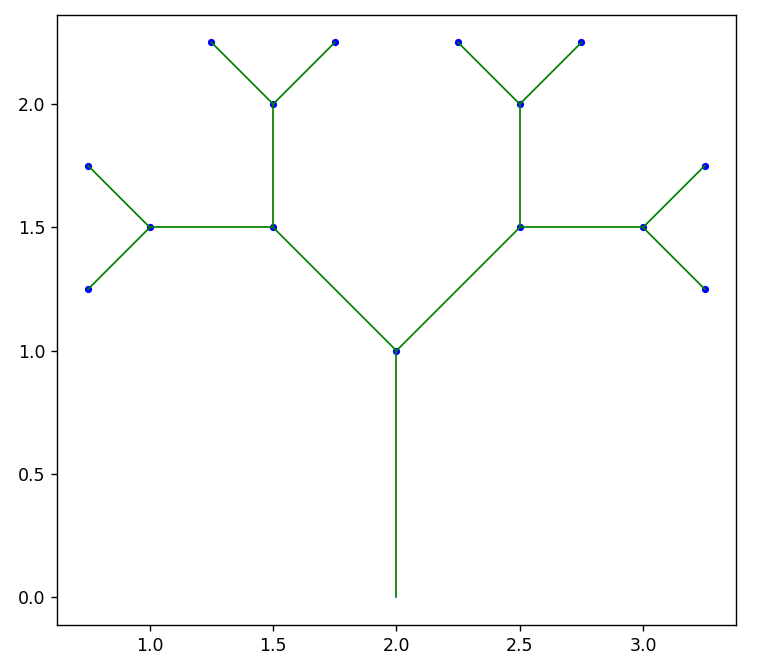
\includegraphics[width=0.6\linewidth]{img/3}
	\caption{Фрактал с глубиной рекурсии 3}
	\label{1}
\end{figure}

\newpage
\begin{figure}[htbp]
	\centering
	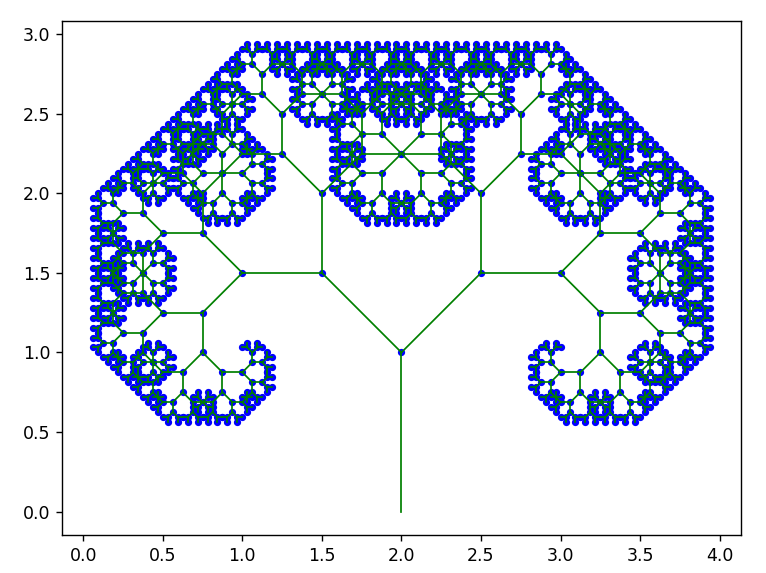
\includegraphics[width=0.6\linewidth]{img/4}
	\caption{Фрактал с глубиной рекурсии 10}
	\label{2}
\end{figure}


Как можно заметить, точки, которые вывела программа, совпадают с точками на \hyperref[1]{рисунке 1}. Это говорит о корректности программы.







\newpage
\section{Задание 2: игра НИМ}
\subsection {Теоретические сведения}

Ним - игра, в которой два игрока по очереди берут предметы, разложенные на несколько кучек. За один ход может быть взято любое количество предметов (больше нуля) из одной кучки. Выигрывает игрок, взявший последний предмет. В классическом варианте игры число кучек равняется трем. В нашем варианте кучка всего одна.

Выигрышной стратегией при таком варианте будут ходы, которые приводят кучу в состояние, когда оставшееся количество камней делится без остатка на (k+1), так как при таком состоянии мы сможем оставлять противнику позиции, в которых ему придется оставлять нам по итогу как минимум один камень. Если же к нашему ходу количество камней уже делится без остатка на (k+1), то мы находимся в проигрышной позиции и не сможем изменить ход игры, если противник не ошибется.

\subsection{Реализация}

Ниже приведен код, на языке Haskell, реализующий игру НИМ с параметрами которые необходимо ввести пользователю при запуске программы (N -- количество камней в куче и K -- ограничение на взятие камней за ход). Во время работы программы каждый ход пользователю пишется, сколько взял бот камней, и спрашивают сколько он собирается взять.

\begin{lstlisting}
{-# LANGUAGE FlexibleContexts #-}

type Step = (String,Int)
type Steps = [Step]


botStep :: (Int, Int, Int) -> (Int, Int, Int) -- (n, k, count)
botStep (n, k, count)
	| n < k = (n, k , n)
	| n > k && count == 1 = (n, k, 1) 
	| otherwise = 
		if (n - count) `mod` (k + 1) == 0 then (n, k, count)
		else botStep(n, k, count - 1)


check :: Int -> Int -> IO Int --[k, count]
check k count  = 
	if count > 0 && count <= k then do return count
	else do
		putStrLn ("Ошибка ввода. Попробуйте снова")
		input <- getLine
		let pl = read input :: Int
		check k pl
	

takeFirstOf3 :: (Int, Int, Int) -> Int
takeFirstOf3 (_,_,count) = count

takeFirstOf2 :: (String, Int) -> String
takeFirstOf2 (name,_) = name

step :: (Int, Int, Steps) -> IO (Int, Int, Steps)
step (n, k, history) 
	| n == 0  = do
		if takeFirstOf2(last history) == "Bot" then  
			putStrLn ("Бот выйграл")
		else 
			putStrLn ("Вы выйграли!!")
		return (n, k, history)
	| n > 0 = do
		let bot = takeFirstOf3(botStep (n, k, k))
			botName = "Bot"
			playerName = "Player"
			newn = n - bot 
			newhistory = history ++ [(botName, bot)]
		putStrLn ("Было "++ show n ++". Бот взял " ++ show bot ++ " камня(ей)") 
		if newn == 0 then do
			putStrLn ("Бот выйграл")
			return (newn, k, newhistory)
		else do
			putStrLn ("Сколько камней возьмете вы? В куче сейчас " ++ show newn ++ ", ограничение - " ++ show k)
			input <- getLine
			let pl = read input :: Int
			finalpl <- check k pl
			let newhistory2 = newhistory ++ [(playerName, finalpl)]
			step (newn - finalpl, k, newhistory2)

printLn :: [Step] -> IO()
printLn = mapM_ (\(name, count) -> putStrLn(name ++ ": " ++ show count)) 

main :: IO()
main = do
	putStrLn "Введите количество камней в куче:"
	input <- getLine
	let n = read input :: Int
	putStrLn "Введите ограничение на взятие камней:"
	input2 <- getLine
	let k = read input2 ::Int
	let history =[] :: [Step]
	(n', k',history') <- step (n, k, history)
	putStrLn ""
	putStrLn "История ходов:"
	printLn history'
	

\end{lstlisting}

\subsection{Результаты}
В качестве примера, возьмем количество камней в куче равным 15 (N = 15), ограничение на взятие камней равным 5 (K = 5). Затем на первом нашем ходу возьмем 5 камней, на следующем -- 4, и так далее.

В конце выведется список ходов в игре.

\begin{lstlisting}
	Введите количество камней в куче:
	15
	Введите ограничение на взятие камней:
	5
	Было 15. Бот взял 3 камня(ей)
	Сколько камней возьмете вы? В куче сейчас 12, ограничение - 5
	5
	Было 7. Бот взял 1 камня(ей)
	Сколько камней возьмете вы? В куче сейчас 6, ограничение - 5
	4
	Было 2. Бот взял 2 камня(ей)
	Бот выйграл
	
	История ходов:
	Bot: 3
	Player: 5
	Bot: 1
	Player: 4
	Bot: 2
\end{lstlisting}


\newpage

\section* {Заключение}
\addcontentsline{toc}{section}{Заключение}
В ходе выполнения практической работы были написаны две программы, одна реализует дерево Пифагора, другая -- игру НИМ. Для каждой задачи был сформирован (.hs) файл, содержащий реализацию.

Прогргамма реализующая дерево Пифагора выводит пары координат фрактала на заданную пользователем глубину

Программа реализующая игру НИМ выводит историю ходов. В ней реализована функции реализующие работу стратегии и организующие логику игры. 

\newpage
%\section*{Список литературы}
%\addcontentsline{toc}{section}{Список литературы} % Добавляем раздел в содержание

\begin{thebibliography}{99}

	\bibitem{kurtz2019}
	Курт У. \textit{Программируй на Haskell} / пер. с англ. С. Соловьева. — Москва: ДМК Пресс, 2019. — 384 с.
	
	\bibitem{barnsley1988}
	Barnsley M.F. \textit{Fractals Everywhere}. — Academic Press, 1988. — 394 p. ISBN-13 \href{https://isbnsearch.org/isbn/9780120790616}{978-0-12-079061-6}.

	
	\bibitem{bouton1901}
	Bouton, C.L. Nim, a game with a complete mathematical theory // Annals of Mathematics. — 1901. — Vol. 3, No. 1. — P. 35–39. DOI: \href{https://doi.org/10.2307/1967631}{10.2307/1967631}.

\end{thebibliography}

\addcontentsline{toc}{section}{Список литературы} % Добавляем раздел в содержание

\end{document}
